% this TeX file provides an awesome example of how TeX will make super 
% awesome tables, at the cost of your of what happens when you try to make a
% table that is very complicated.
% Originally turned in for Dr. Nico's Security Class
\documentclass[12pt]{article}



% text shouldn't exceed 6 inch width and 8 inch height
\usepackage[a4paper, total={6in, 8in}, margin=1in]{geometry}

% makes it so that the first paragraph of every section is indented
\usepackage{indentfirst}

% For listing code
\usepackage{listings}

% For lst entries (code)
\lstset{columns=fullflexible, basicstyle=\ttfamily,
    backgroundcolor=\color{white},xleftmargin=0.5cm,frame=tlbr,framesep=4pt,framerule=0pt}
    

\usepackage{titlesec}


% math equation package, "fleqn" positions equations at a fixed indent from the left margin
% math equation leqno brings the numbering for equations to left side
\usepackage{amsmath}

\usepackage{parskip}
\setlength{\parskip}{.8em}

% Set the indent to zero for the whole document
\setlength\parindent{0pt}





% For graphics/images
\usepackage{graphicx}



% For captions under images
\usepackage{caption}

% float package for image alignment
\usepackage{float}
% images are in the directory images/
\graphicspath{ {images/} }

% \usepackage{pagecolor}% With option pagecolor={somecolor or none}
% \definecolor{ultramarine}{RGB}{253,255,244} 

% degree symbol: \degree
\usepackage{gensymb}



\begin{document}

% \pagecolor{ultramarine}



\begingroup  
  \centering
  \LARGE \textbf{Internal Positioning System (IPS) Application For Android\\[0.4em]}
  \large Andre Bododea \\[0.2em]
  \large s1350924 \par

\endgroup


\section*{Introduction}

\cite{kaemarungsi2004modeling}

A compass application was requested by the customer. The main feature required was that the application includes a visual compass which rotates depending on the direction the phone is facing. It must also display the direction from $0\degree$ to $360\degree$. Anything past these two main features is left to the discretion of the engineer. This guide will begin be organized by first explaining the control flow, then it will go on to discuss the main compass feature, and finally the extra features will be discussed.

\section*{Control Flow}

The user is presented with a start when he first opens up the application (\textbf{fig 1}). This gives him the option to choose either the compass feature or the camera feature. If he chooses the compass feature (\textbf{fig 2}), he has access to the rotating compass and the direction in degrees relative to $0\degree$ (North).


\begin{figure}[!htb]
    \centering
    \begin{minipage}[b]{.3\textwidth} 
        \centering  
        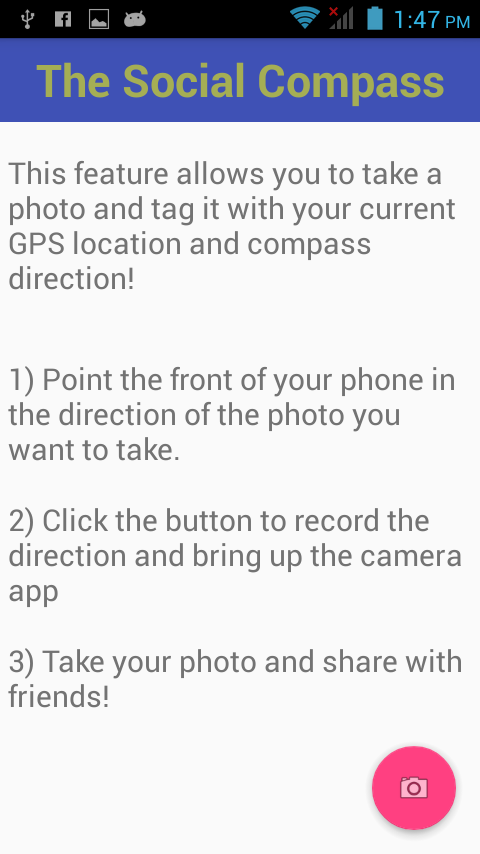
\includegraphics[scale=1.2, width=\linewidth]{photo1.png}     
        \caption{Start screen}  
    \end{minipage}    
    \hfill
    \begin{minipage}[b]{.3\textwidth}  
        \centering  
        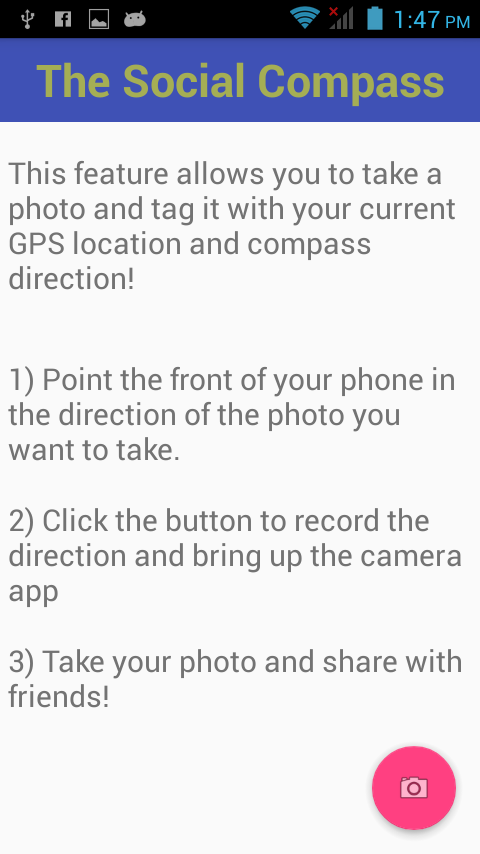
\includegraphics[scale=1.2, width=\linewidth]{photo1.png}  
        \caption{Compass screen}  
    \end{minipage} 
    \hfill
    \begin{minipage}[b]{.3\textwidth}  
        \centering  
        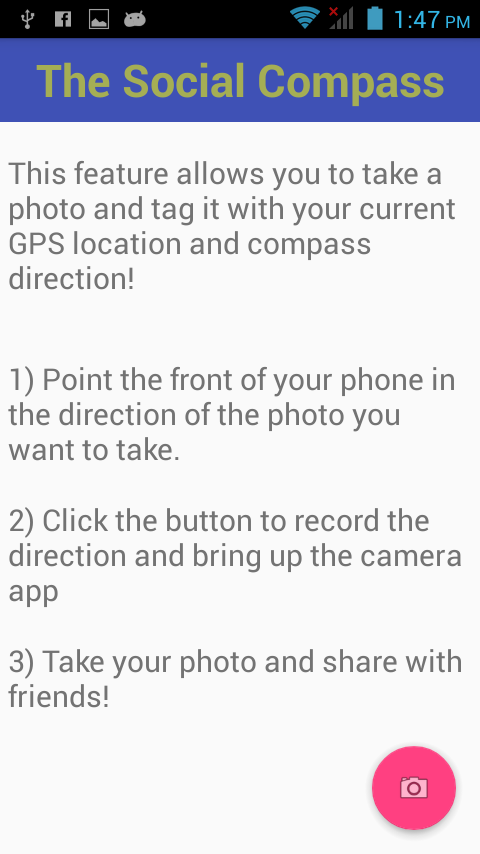
\includegraphics[scale=1.2, width=\linewidth]{photo1.png}  
        \caption{Camera intro}  
    \end{minipage}  
\end{figure}


If the user chooses the camera (\textbf{fig 3}), he is presented with instructions. The user can then click the camera button and proceed to the camera app (\textbf{fig 4}). Once the user takes a photo, the photo is then saved and the user is presented with the option to share the photo they just took (\textbf{fig 5}). The user may then choose to share the photo, which is now tagged with their latitude, longitude, and current direction (\textbf{fig 6}). Sharing via Facebook, text, email, and any other installed app is supported.



\section*{Compass Feature}

\textbf{CompassActivity}

The sensors used in the compass (\textbf{fig 2}) are the magnetometer and accelerometers. They are implemented via two listeners, one for each. Any time the values are changed, the onSensorChanged() function is called and the sensor values are passed to arrays. These values are then passed to the calculateOrientation() method which was designed by me. The built-in SensorManager.getRotationMatrix() function is used with the accelerometer and magnetometer values, then the SensorManager.getOrientation() function to convert to degrees between . That value is then transformed to a range between 0 and 360 to calculate the degrees respective to  (magnetic North).

The visual compass is an image that is rotated via the RotateAnimation() function. This simply takes an image and rotates it based on the number of degrees calculated as discussed previously. In order to prevent erratic and shaky movements, a low-pass filter is applied in order to smooth the motion of the image. The function is written as such: $ \verb!magnetic_field_x! = \alpha \times \verb!previous_magnetic_field_x! + (1 - \alpha) \times \verb!current_magnetic_field_x! $ where $\alpha = 0.7$ for this application.



\section*{Extra Features}

\textbf{CameraActivity}

The extra feature implemented is a camera with tagging and sharing features. An onClickListener() is used to wait for the button press in (\textbf{fig 3)}. When this method is called, it starts a camera intent (\textbf{fig 4}), and creates a URI where the produced photo is saved. Immediately thereafter, a message is displayed that acknowledges the success of the photo taking. Then the custom function overlayPhoto() is called, which transforms the photo at the given URI into a bitmap. 

It then puts that bitmap into a Canvas object and uses the Paint object to write the coordinates and the direction over the bitmap. This bitmap is then saved as a JPEG file at the same URI where it was read from and shared via startActivity(Intent.createChooser(shareIntent, "Share images to..")); (\textbf{fig 5}). The user can choose an app to share with and share the tagged photo. (\textbf{fig 6}) 


\begin{figure}[H]
    \centering
    \begin{minipage}[b]{.3\textwidth} 
        \centering  
        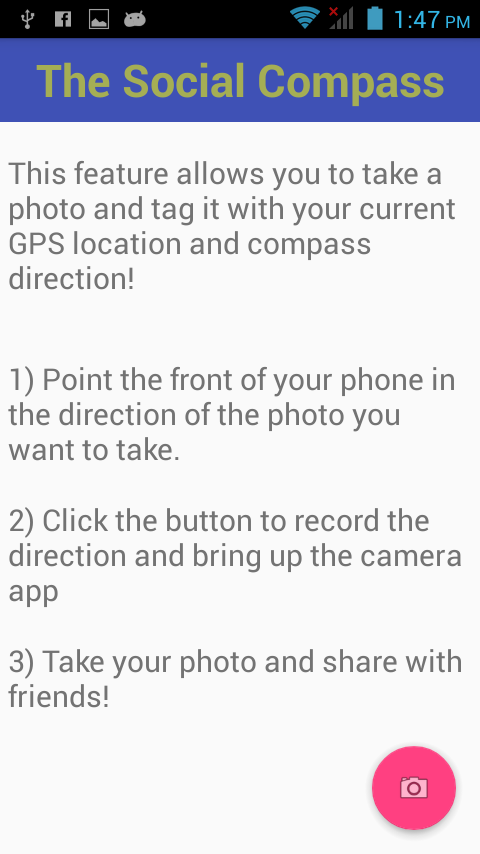
\includegraphics[scale=1.2, width=\linewidth]{photo1.png}     
        \caption{Photo capture}  
    \end{minipage}    
    \hfill
    \begin{minipage}[b]{.3\textwidth}  
        \centering  
        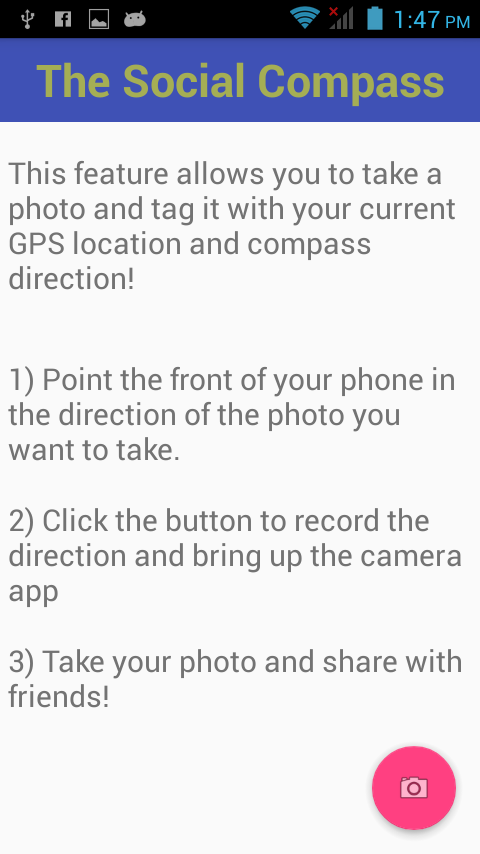
\includegraphics[scale=1.2, width=\linewidth]{photo1.png}  
        \caption{Share photo}  
    \end{minipage} 
    \hfill
    \begin{minipage}[b]{.3\textwidth}  
        \centering  
        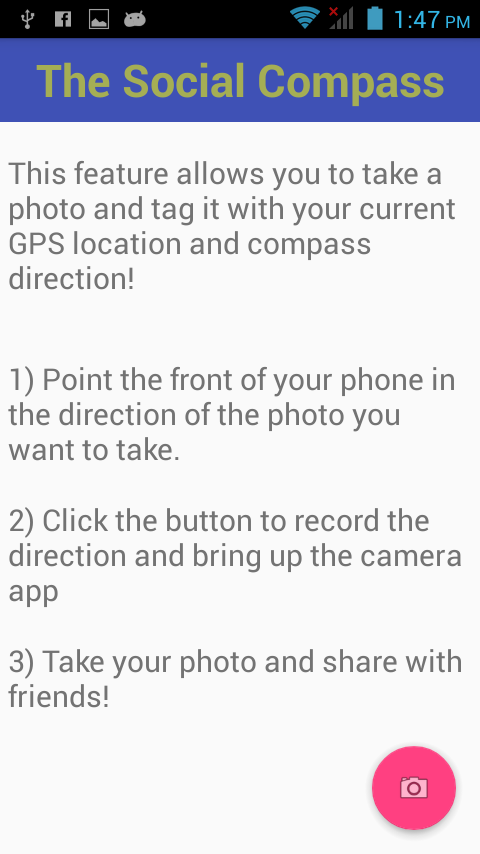
\includegraphics[scale=1.2, width=\linewidth]{photo1.png}  
        \caption{Facebook sharing}  
    \end{minipage}  
\end{figure}




\vspace{\baselineskip}

\bibliographystyle{unsrt}
\bibliography{es2}


\end{document}


